\part{Problème de satisfaction de contraintes CSP}
\pagebreak

\chapter{Introduction et modèles}
\pagebreak

Une Solution d'un problème CSP est une assignation d'une valeur à chaque variables de P tel que toutes les contraintes de P soit satisfaite.\\

\section{exemple simple}

Trouver une assignation Minimal et Maximal pour chaque variables de P dans le problème suivant:\\
\begin{description}
\item[vars(P)] = $w,x,y,z$
\item[Dom(P)]\  \begin{description}
\item[Dom(w,x)] = $\{1,2,3\}$
\item[Dom(y,z)] = $range(4)$
\end{description}
\item[Contraintes]\  \begin{description}
\item[$~$] $w = x$
\item[$~$] $x \leq y + 1$
\item[$~$] $y > z$
\item[$~$] $(x,z) \in \{(1,2),(2,1),(2,4),(3,3)\}$
\end{description}
\end{description}
\ \\
Une solution serait:
\begin{description}
\item[Minimal] $w=x=1, y=3, z=2$
\item[Maximal] $w=x=z=3, y=4$
\end{description}

\pagebreak
\subsection{Graphe de contraintes}

Chaque variable est un nœud et chaque contraintes est représenté par une arête entre les variables concerné.\\
\begin{center}
\begin{tikzpicture}[-,>=stealth',shorten >=1pt,auto,node distance=2.8cm,
                    semithick]
  \tikzstyle{every state}=[fill=white,draw=none,text=black]

  \node[state]         (W)                    {$W$};
  \node[state]         (X) [left of=W]        {$X$};
  \node[state]         (Y) [below right of=X] {$Y$};
  \node[state]		   (Z) [below left of=X]  {$Z$};
  

  \path (X) edge              node {} (W)
            edge              node {} (Y)
            edge			  node {} (Z)
        (Z) edge			  node {} (Y);
\end{tikzpicture}
\end{center}
\subsection{Graphe de compatibilité}

Représenter toutes variables avec des ensemble contenant toutes les valeur de leurs domaine puis relier chaque éléments de l'ensemble avec un autre tel que les contraintes ne soit pas violet:\\
\begin{center}
\includegraphics[scale=0.6]{img/aic_csp_1.jpg} 
\end{center}

\chapter{Filtrage}
\pagebreak
\section{Filtrage du domaine via les contraintes}

Un problème peut être définit comme une intersection de sous problème à qui un sous problème est représenté par un filtre du domaine des variable et une contrainte qui va réduire le domaine des variable à un étant de consistance peu importe les valeurs des variables.\\

\begin{description}
\item[Arc Consistency (AC)] Tous les valeurs inconsistant sont identifié et retiré
\item[Bound Consistency (BC)] Les valeurs inconsistant sont les bornes des domaine et ils sont identifié et retiré
\end{description}

\subsection{Exemple}

\formula{Contrainte $w + 3 = z$}
Avec
\formula{$dom(w) = \{1,3,4,5\}$}
\formula{$dom(z) = \{4,5,8\}$}

Avec un filtre AC:\\
\formula{$dom(w) = \{1,5\}$ et $dom(z) = \{4,8\}$}

Avec un filtre BC:\\
\formula{$dom(w) = \{1,3,4,5\}$ et $dom(z) = \{4,5,8\}$}

\pagebreak
\section{Notion de Support}
Soit $c_{xyz}$ une contrainte tel que $c_{xyz}$ égal:
\formula{$dom(x,y) = \{a,b\} et dom(z) = \{b,c\}$}

On n'a $T = rel(c_{xyz})$ et V = $dom(x)$ x $dom(y)$ x $dom(z)$:\\

\begin{multicols}{2}
[$\cvert{(z,b)}$ a un support mais $\crouge{(z,c)}$ n'en n'a pas]

\begin{tabular}{|ccc|}
\hline $ $ & T & $ $\\
\hline
a & a & a \\
$\cvert{a}$ & $\cvert{b}$ & $\cvert{b}$\\
$\crouge{a}$ & $\crouge{c}$ & $\crouge{c}$\\
 b & a & a \\ b & b & b \\
c & a & a \\
$\crouge{c}$ & $\crouge{c}$ & $\crouge{c}$\\
\hline
\end{tabular}

\begin{tabular}{|ccc|}
\hline $ $ & V & $ $\\
\hline
a&a&b\\
$\crouge{a}$&$\crouge{a}$&$\crouge{c}$\\
$\cvert{a}$&$\cvert{b}$&$\cvert{b}$\\
$\crouge{a}$&$\crouge{b}$&$\crouge{c}$\\
b&a&b\\
$\crouge{b}$&$\crouge{a}$&$\crouge{c}$\\
b&b&b\\
$\crouge{b}$&$\crouge{b}$&$\crouge{c}$\\
\hline
\end{tabular}
\end{multicols}
\pagebreak
\section{AC filtre AllDifferent}

\begin{multicols}{2}
[Soit un sudoku block avec la contrainte $allDifferent(w,x,y,z)$:]
\begin{tabular}{|c|c|c|}
\hline $\cvert{3}$ & w & $\cvert{6}$\\
\hline x & $\cvert{8}$ & y\\
\hline $\cvert{1}$ & $\cvert{4}$ & z\\
\hline
\end{tabular}
\begin{description}
\item[w] = \{2,5\}
\item[x] = \{5,7,9\}
\item[y] = \{7\}
\item[z] = \{2,5\}
\end{description}
\end{multicols}

\begin{multicols}{2}
[Dans ce cas, y contient un singleton, donc il sera trivialement résolut en affectant y = 7 et en suppriment tout les occurrences de 7 dans les autres variables:]
\begin{tabular}{|c|c|c|}
\hline 3 & w & 6\\
\hline x & 8 & $\cvert{7}$\\
\hline 1 & 4 & z\\
\hline
\end{tabular}
\begin{description}
\item[w] = \{2,5\}
\item[x] = \{5,$\crouge{7}$,9\}
\item[z] = \{2,5\}
\end{description}
\end{multicols}

\begin{multicols}{2}
[nous pouvons construire le Hall sets suivant: $(w,z) vs (2,5)$ et donc supprimer toutes les occurrences de 2 et 5 dans les autres variables:]
\begin{tabular}{|c|c|c|}
\hline 3 & w & 6\\
\hline $\cvert{9}$ & 8 & 7\\
\hline 1 & 4 & z\\
\hline
\end{tabular}
\begin{description}
\item[w] = \{2,5\}
\item[x] = \{$\crouge{5}$,9\}
\item[z] = \{2,5\}
\end{description}
\end{multicols}

\begin{multicols}{2}
[Ce qui nous donne 2 solutions, (w=2,z=5) ou (w=5,z=2)]
\begin{tabular}{|c|c|c|}
\hline 3 & w & 6\\
\hline 9 & 8 & 7\\
\hline 1 & 4 & z\\
\hline
\end{tabular}
\begin{description}
\item[w] = \{2,5\}
\item[z] = \{2,5\}
\end{description}
\end{multicols}
\pagebreak

\begin{multicols}{2}
[Soit un autre exemple plus complexe avec une contrainte $allDifferent(u,v,w,x,y,z)$ et un domaine $\{1,2,5,6,7,9\}$:]
\begin{description}
\item[u] = \{1,2\}
\item[v] = \{2,9\}
\item[w] = \{1,5,6\}
\item[x] = \{2,6\}
\item[y] = \{6,7,9\}
\item[z] = \{1,9\}
\end{description}
\end{multicols}

\begin{multicols}{2}
[On peut crée une Hall sets de taille 3 $(u,v,z)=(1,2,9)$ et éliminer toutes les occurrences de 1,2,9 dans les autres variables:]
\begin{description}
\item[u] = \{1,2\}
\item[v] = \{2,9\}
\item[w] = \{5,6\}
\item[x] = \{6\}
\item[y] = \{6,7\}
\item[z] = \{1,9\}
\end{description}
\end{multicols}

\begin{multicols}{2}
[On peut affecter x à 6 et supprimer toutes les occurrences de 6 dans les autres variables:]
\begin{description}
\item[u] = \{1,2\}
\item[v] = \{2,9\}
\item[w] = 5
\item[x] = 6
\item[y] = 7
\item[z] = \{1,9\}
\end{description}
\end{multicols}

\begin{multicols}{2}
[On obtient donc la tableau suivant qui pour n'importe quelle valeurs de u,v,w,x,y,z donne:]
\begin{tabular}{cccccc}
u&v&w&x&y&z\\ \hline 1&2&5&6&7&1\\ 2&9&$ $&$ $&$ $&9\\
\end{tabular}
\end{multicols}
\pagebreak
\section{AC filtre Cardinalité}

Une contrainte de cardinalité note $cardinality(X,Y,L,U)$ qui a $X$ est l'ensemble des variables, $Y$ le domaine des variables de $X$, $(L_i,U_i)$ le range d'occurrences de la variable $Y_i$ dans tout le modèle.\\
Si $(L_i=1,U_i=3)$ alors la variable $Y_i$ ne pourra être présent de 1 à 3 fois maximum, si $(L_i=2,U_i=2)$ alors la variable $Y_i$ devra être présent 2 fois.\\

Prenons:
\begin{description}
\item[X] les agents \{Peter,Paul,Mary,John,Bob,Mike,Julia\}
\item[Y] les activités \{Morning (M),Day (D),Night (N),Backup (B),Off (O)\}
\item[L] \{1,1,1,0,0\}
\item[U] \{2,2,1,2,2\}
\end{description}

Nous voudrons réduire ce genre de tableau suivant:\\
\begin{tabular}{c|ccccccc}
$ $&Monday&Tuesday&Wendsday&Thursday&Friday&Saturday&Sunday\\ \hline
Peter&D&N&N&N&O&O&O\\
Paul&O&O&D&D&M&M&B\\
Mary&M&M&D&D&O&O&N\\
\end{tabular}

\begin{center} \scalebox{0.8}{
\begin{tikzpicture}[-,>=stealth',shorten >=1pt,auto,node distance=2cm,
                    semithick]
  \tikzstyle{every state}=[fill=white,draw=none,text=black]

  \node[state]         (PETER)                  {$Peter$};
  \node[state]         (PAUL) [right of=PETER]  {$Paul$};
  \node[state]         (MARY) [right of=PAUL]   {$Mary$};
  \node[state]         (JOHN) [right of=MARY]   {$John$};
  \node[state]         (BOB)  [right of=JOHN]   {$Bob$};
  \node[state]         (MIKE) [right of=BOB]    {$Mike$};
  \node[state]         (JULIA)[right of=MIKE]   {$Julia$};
  \node[state]         (NONE)[below right of=PETER] {$ $};
  \node[state]         (M)[below right of=NONE]{$M(1,2)$};
  \node[state]         (D)[right of=M]          {$D(1,2)$};
  \node[state]         (N)[right of=D]          {$N(1,1)$};
  \node[state]         (B)[right of=N]          {$B(0,2)$};
  \node[state]         (O)[right of=B]          {$O(0,2)$};

  \path (M) edge node {} (PETER)
            edge node {} (PAUL)
            edge node {} (MARY)
            edge node {} (JOHN)
            edge node {} (BOB)
        (D) edge node {} (PETER)
            edge node {} (PAUL)
            edge node {} (JOHN)
            edge node {} (BOB)
            edge node {} (MIKE)
        (N) edge node {} (BOB)
            edge node {} (MIKE)
            edge node {} (JULIA)
        (B) edge node {} (MIKE)
        (O) edge node {} (MIKE)
            edge node {} (JULIA);
\end{tikzpicture}}
\end{center}

On peut assigner $Bob$ à la tache $N$ et assigner à $Julia$ la tache $O$, le reste sera des combinaison possible:
\begin{center} \scalebox{0.8}{
\begin{tikzpicture}[-,>=stealth',shorten >=1pt,auto,node distance=2cm,
                    semithick]
  \tikzstyle{every state}=[fill=white,draw=none,text=black]

  \node[state]         (PETER)                  {$Peter$};
  \node[state]         (PAUL) [right of=PETER]  {$Paul$};
  \node[state]         (MARY) [right of=PAUL]   {$Mary$};
  \node[state]         (JOHN) [right of=MARY]   {$John$};
  \node[state]         (BOB)  [right of=JOHN]   {$Bob$};
  \node[state]         (MIKE) [right of=BOB]    {$Mike$};
  \node[state]         (JULIA)[right of=MIKE]   {$Julia$};
  \node[state]         (NONE)[below right of=PETER] {$ $};
  \node[state]         (M)[below right of=NONE]{$M(1,2)$};
  \node[state]         (D)[right of=M]          {$D(1,2)$};
  \node[state]         (N)[right of=D]          {$N(1,1)$};
  \node[state]         (B)[right of=N]          {$B(0,2)$};
  \node[state]         (O)[right of=B]          {$O(0,2)$};

  \path (M) edge node {} (PETER)
            edge node {} (PAUL)
            edge node {} (MARY)
            edge node {} (JOHN)
        (D) edge node {} (PETER)
            edge node {} (PAUL)
            edge node {} (JOHN)
        (N) edge node {} (BOB)
        (B) edge node {} (MIKE)
        (O) edge node {} (MIKE)
            edge node {} (JULIA);
\end{tikzpicture}}
\end{center}

\section{AC filtre Sum à une borne}

Soit un filtre $sum$ avec les variables $(x,y,z,a,b,c)$ dans le domaine $range(1,5)$ appliqué sur l'équation:
\formula{$2x+3y+2z+a+4b+2c \geq 50$}
\begin{center}
\begin{tabular}{cccccc}
x&y&z&a&b&c\\ \hline
1&1&1&1&1&1\\ 2&2&2&2&2&2\\ 3&3&3&3&3&3\\ 4&4&4&4&4&4\\
\end{tabular}
\end{center}
Si le somme des maximums de chaque variable ne respecte pas la contrainte, alors il n'existe aucun assignement des variables tel que la contrainte serait satisfaite:
\formula{$2*4+3*4+2*4+4+4*4+2*4 = 8+12+8+4+16+8 = 56 \geq 50$}
Pour chaque variables, enlever son impacte dans le résultat précédemment obtenue et refaire l'opération de dépilé avec les différents $x$ tant que un $x_i$ ne satisfait pas la contrainte:\\
\ \\
Pour x:
\begin{description}
\item[] $2*4+3*4+2*4+4+4*4+2*4 = 8+12+8+4+16+8 = 56 \geq 50$
\item[] $ 56 - 2*4 + 2*1 = 50 \geq 50$, donc $x=1$ fonctionne
\item[] (pareil pour z,c)
\end{description}
\ \\
Pour y:
\begin{description}
\item[] $ 56 - 3*4 + 3*1 = 44 \geq 50$, donc $y=1$  ne fonctionne pas
\item[] $ 56 - 3*4 + 3*2 = 50 \geq 50$, donc $y=2$  fonctionne
\end{description}
\pagebreak
Pour b:
\begin{description}
\item[] $ 56 - 4*4 + 4*1 = 40 \geq 50$, donc $b=1$  ne fonctionne pas
\item[] $ 56 - 4*4 + 4*2 = 44 \geq 50$, donc $b=2$  ne fonctionne pas
\item[] $ 56 - 4*4 + 4*3 = 50 \geq 50$, donc $b=3$  fonctionne
\end{description}
\ \\
On obtient:\\
\begin{center}
\begin{tabular}{cccccc}
x&y&z&a&b&c\\ \hline
1&$ $&1&1&$ $&1\\ 2&2&2&2&$ $&2\\ 3&3&3&3&3&3\\ 4&4&4&4&4&4\\
\end{tabular}
\end{center}

\pagebreak
\section{AC filtre avec Sum à deux bornes}

\begin{multicols}{3}
[Soit $x,y,z$ avec comme domaine $dom(x)=dom(y)=dom(z) = {1,2}$ et avec une contrainte $8 \leq 2x + 2y + z \leq 9$.\\
Via résolution graphique on obtient et réduit le graphe comme ceci:]

\scalebox{0.8}{
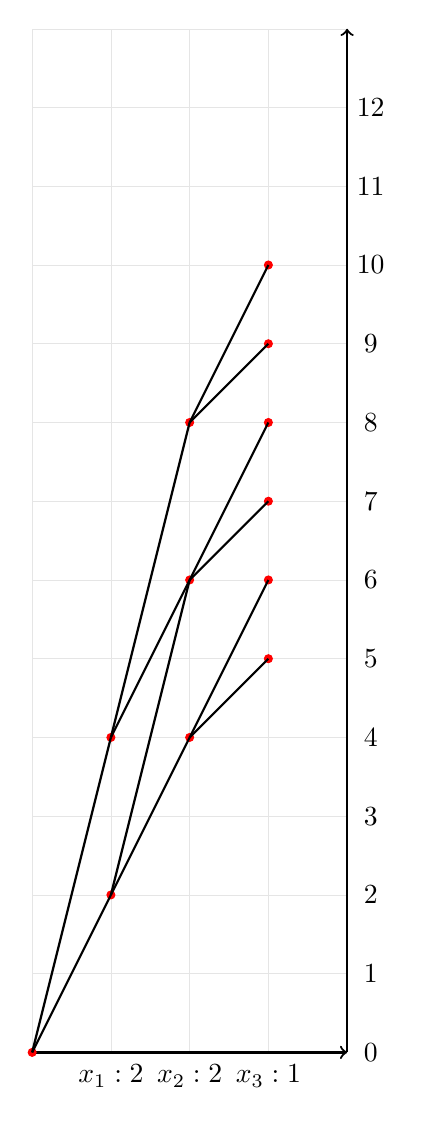
\begin{tikzpicture}
 \draw[help lines, gray!20] (0,0) grid (4,13);
 
 \node at (1,-0.3) {$x_1:2$};
 \node at (2,-0.3) {$x_2:2$};
 \node at (3,-0.3) {$x_3:1$};

 \draw [->, thick] (0,0) -- (4,0);
 \draw [->, thick] (4,0) -- (4,13);
 
 \foreach \vec in {0,1,2,3,4,5,6,7,10,11,12}{
 	\node at (4.3,\vec) {$\vec$};
 }
 
  \foreach \vec in {8,9}{
 	\node at (4.3,\vec) {$\cblue{\vec}$};
 }
 
 \foreach \vec in {(0,0),(1,2),(1,4),(2,4),(2,6),(2,8),(3,5),(3,6),(3,7),(3,8),(3,9),(3,10)}{
 	\draw [fill, red] \vec circle [radius=0.05];
 }
 
 \draw [thick, black] (0,0) -- (1,2);
 \draw [thick, black] (0,0) -- (1,4);
 \draw [thick, black] (1,2) -- (2,4);
 \draw [thick, black] (1,2) -- (2,6);
 \draw [thick, black] (1,4) -- (2,6);
 \draw [thick, black] (1,4) -- (2,8);
 \draw [thick, black] (2,4) -- (3,5);
 \draw [thick, black] (2,4) -- (3,6);
 \draw [thick, black] (2,6) -- (3,7);
 \draw [thick, black] (2,6) -- (3,8);
 \draw [thick, black] (2,8) -- (3,9);
 \draw [thick, black] (2,8) -- (3,10);
 
\end{tikzpicture}}

\scalebox{0.8}{
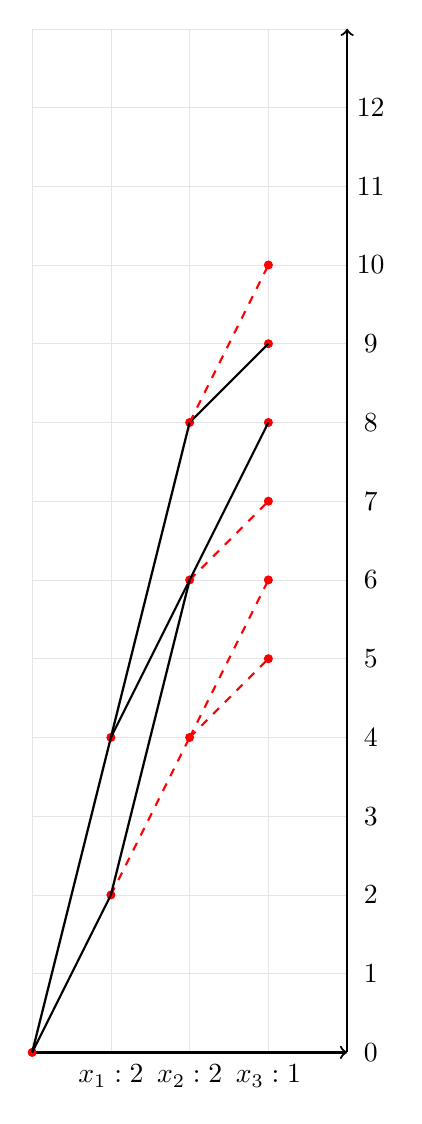
\begin{tikzpicture}
 \draw[help lines, gray!20] (0,0) grid (4,13);
 
 \node at (1,-0.3) {$x_1:2$};
 \node at (2,-0.3) {$x_2:2$};
 \node at (3,-0.3) {$x_3:1$};

 \draw [->, thick] (0,0) -- (4,0);
 \draw [->, thick] (4,0) -- (4,13);
 
 \foreach \vec in {0,1,2,3,4,5,6,7,10,11,12}{
 	\node at (4.3,\vec) {$\vec$};
 }
 
  \foreach \vec in {8,9}{
 	\node at (4.3,\vec) {$\cblue{\vec}$};
 }
 
 \foreach \vec in {(0,0),(1,2),(1,4),(2,4),(2,6),(2,8),(3,5),(3,6),(3,7),(3,8),(3,9),(3,10)}{
 	\draw [fill, red] \vec circle [radius=0.05];
 }
 
 \draw [thick, black] (0,0) -- (1,2);
 \draw [thick, black] (0,0) -- (1,4);
 \draw [thick, dashed, red] (1,2) -- (2,4);
 \draw [thick, black] (1,2) -- (2,6);
 \draw [thick, black] (1,4) -- (2,6);
 \draw [thick, black] (1,4) -- (2,8);
 \draw [thick, dashed, red] (2,4) -- (3,5);
 \draw [thick, dashed, red] (2,4) -- (3,6);
 \draw [thick, dashed, red] (2,6) -- (3,7);
 \draw [thick, black] (2,6) -- (3,8);
 \draw [thick, black] (2,8) -- (3,9);
 \draw [thick, dashed, red] (2,8) -- (3,10);
 
\end{tikzpicture}}

\scalebox{0.8}{
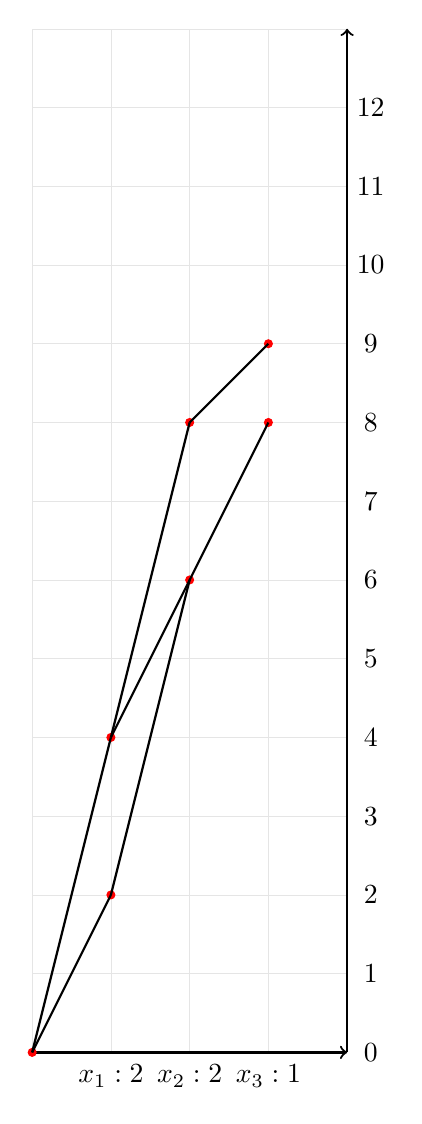
\begin{tikzpicture}
 \draw[help lines, gray!20] (0,0) grid (4,13);
 
 \node at (1,-0.3) {$x_1:2$};
 \node at (2,-0.3) {$x_2:2$};
 \node at (3,-0.3) {$x_3:1$};

 \draw [->, thick] (0,0) -- (4,0);
 \draw [->, thick] (4,0) -- (4,13);
 
 \foreach \vec in {0,1,2,3,4,5,6,7,10,11,12}{
 	\node at (4.3,\vec) {$\vec$};
 }
 
  \foreach \vec in {8,9}{
 	\node at (4.3,\vec) {$\cblue{\vec}$};
 }
 
 \foreach \vec in {(0,0),(1,2),(1,4),(2,6),(2,8),(3,8),(3,9)}{
 	\draw [fill, red] \vec circle [radius=0.05];
 }
 
 \draw [thick, black] (0,0) -- (1,2);
 \draw [thick, black] (0,0) -- (1,4);
 \draw [thick, black] (1,2) -- (2,6);
 \draw [thick, black] (1,4) -- (2,6);
 \draw [thick, black] (1,4) -- (2,8);
 \draw [thick, black] (2,6) -- (3,8);
 \draw [thick, black] (2,8) -- (3,9);
 
\end{tikzpicture}}
\end{multicols}

Dans un premier temps on représente toutes les possibilités, dans un second temps on élimine récursivement tout les feuille de l'arbre qui pointe sur des noeuds hors objectif (dans notre cas hors de 8,9). Toutes les branches seul qui ne sont pas relié aux bornes 8 et 9 seront supprimé.\\
On peut attribuer au variables toutes les possibilités de chemin de l'arbre:
\begin{description}
\item[] $x_1=1, x_2=2, x_3=1$ : $1*2 + 2*2 + 1*2 = 8$
\item[] $x_1=2, x_2=2, x_3=1$ : $2*2 + 2*2 + 1*1 = 9$
\end{description}
\pagebreak

\chapter{Recherche de réponses}
Selon les problèmes, l'arbre de décision peut être assez profond / large à explorer, on peut inféré sur les contraintes par filtrage ou par propagation pour ne pas à avoir à explorer certains sous arbres.
\pagebreak

\section{recherche avec backtrack}
Tout dépend du niveau de l'algorithme de filtrage utilisé, en utilisant $look-ahead$ algorithme on obtient:
\begin{description}
\item[BT] $ $
\item[FC] (Forward Checking)
\item[MAC] (Maintaining Arc Consistency)
\end{description}

Pour l'algorithme $look-back$ effectuant des choses plus intelligente:
\begin{description}
\item[CBJ] (Conflict-directed backjumping)
\item[DBT] (Dynamic Backtracking)
\end{description}

\pagebreak
\subsection{BT}
BT est le plus simple, pour chaque node, on va regarder si celui ci satisfait toutes les contraintes.
Sur le problème des N-queens=4:
\begin{multicols}{3}
\scalebox{0.9}{
\begin{tabular}{c|c|c|c}
$ $&$X$&$ $&$ $\\\hline
$ $&$ $&$ $&$ $\\\hline
$ $&$ $&$ $&$ $\\\hline
$X$&$ $&$ $&$ $\\
\end{tabular}
}
\scalebox{0.9}{
\begin{tabular}{c|c|c|c}
$ $&$X$&$ $&$ $\\\hline
$ $&$ $&$ $&$ $\\\hline
$ $&$ $&$ $&$ $\\\hline
$\crouge{X}$&$ $&$\crouge{X}$&$ $\\
\end{tabular}
}
\scalebox{0.9}{
\begin{tabular}{c|c|c|c}
$ $&$X$&$ $&$ $\\\hline
$ $&$ $&$ $&$ $\\\hline
$ $&$ $&$X$&$ $\\\hline
$X$&$ $&$ $&$ $\\
\end{tabular}
}
\end{multicols}

\begin{multicols}{3}
\scalebox{0.9}{
\begin{tabular}{c|c|c|c}
$ $&$X$&$ $&$ $\\\hline
$ $&$ $&$ $&$ $\\\hline
$ $&$ $&$X$&$ $\\\hline
$\crouge{X}$&$ $&$ $&$\crouge{X}$\\
\end{tabular}
}
\scalebox{0.9}{
\begin{tabular}{c|c|c|c}
$ $&$X$&$ $&$ $\\\hline
$ $&$ $&$ $&$ $\\\hline
$ $&$ $&$\crouge{X}$&$\crouge{X}$\\\hline
$X$&$ $&$ $&$ $\\
\end{tabular}
}
\scalebox{0.9}{
\begin{tabular}{c|c|c|c}
$ $&$X$&$ $&$ $\\\hline
$ $&$ $&$ $&$\crouge{X}$\\\hline
$ $&$ $&$\crouge{X}$&$ $\\\hline
$X$&$ $&$ $&$ $\\
\end{tabular}
}
\end{multicols}

\begin{multicols}{3}
\scalebox{0.9}{
\begin{tabular}{c|c|c|c}
$ $&$X$&$ $&$\crouge{X}$\\\hline
$ $&$ $&$ $&$ $\\\hline
$ $&$ $&$X$&$ $\\\hline
$\crouge{X}$&$ $&$ $&$ $\\
\end{tabular}
}
\scalebox{0.9}{
\begin{tabular}{c|c|c|c}
$ $&$X$&$ $&$ $\\\hline
$ $&$ $&$\crouge{X}$&$ $\\\hline
$ $&$ $&$ $&$ $\\\hline
$\crouge{X}$&$ $&$ $&$ $\\
\end{tabular}
}
\scalebox{0.9}{
\begin{tabular}{c|c|c|c}
$ $&$\crouge{X}$&$\crouge{X}$&$ $\\\hline
$ $&$ $&$ $&$ $\\\hline
$ $&$ $&$ $&$ $\\\hline
$X$&$ $&$ $&$ $\\
\end{tabular}
}
\end{multicols}

\begin{multicols}{3}
\scalebox{0.9}{
\begin{tabular}{c|c|c|c}
$ $&$ $&$ $&$ $\\\hline
$ $&$ $&$ $&$ $\\\hline
$X$&$ $&$ $&$ $\\\hline
$ $&$ $&$ $&$ $\\
\end{tabular}
}
\scalebox{0.9}{
\begin{tabular}{c|c|c|c}
$ $&$ $&$ $&$ $\\\hline
$ $&$ $&$ $&$ $\\\hline
$\crouge{X}$&$ $&$ $&$ $\\\hline
$ $&$\crouge{X}$&$ $&$ $\\
\end{tabular}
}
\scalebox{0.9}{
\begin{tabular}{c|c|c|c}
$ $&$ $&$ $&$ $\\\hline
$ $&$ $&$ $&$ $\\\hline
$\crouge{X}$&$\crouge{X}$&$ $&$ $\\\hline
$ $&$ $&$ $&$ $\\
\end{tabular}
}
\end{multicols}
\pagebreak

\subsection{FC}
FC, toutes les nodes utilisé réduire le domaine des autres nodes, si un domaine est vide, plus besoin de continuer il n'y a pas de solution:
Sur le problème des N-queens=4:
\begin{multicols}{3}
\scalebox{0.9}{
\begin{tabular}{c|c|c|c}
$ $&$ $&$ $&$\crouge{\#}$\\\hline
$ $&$ $&$\crouge{\#}$&$ $\\\hline
$ $&$\crouge{\#}$&$ $&$ $\\\hline
$X$&$\crouge{\#}$&$\crouge{\#}$&$\crouge{\#}$\\
\end{tabular}
}
\scalebox{0.9}{
\begin{tabular}{c|c|c|c}
$ $&$ $&$\crouge{\#}$&$\crouge{\#}$\\\hline
$ $&$X$&$\crouge{\#}$&$\crouge{\#}$\\\hline
$ $&$\crouge{\#}$&$ $&$ $\\\hline
$X$&$\crouge{\#}$&$\crouge{\#}$&$\crouge{\#}$\\
\end{tabular}
}
\scalebox{0.9}{
\begin{tabular}{c|c|c|c}
$ $&$ $&$ $&$\crouge{\#}$\\\hline
$ $&$\crouge{\#}$&$\crouge{\#}$&$ $\\\hline
$ $&$\crouge{\#}$&$ $&$ $\\\hline
$X$&$\crouge{\#}$&$\crouge{\#}$&$\crouge{\#}$\\
\end{tabular}
}
\end{multicols}

\begin{multicols}{3}
\scalebox{0.9}{
\begin{tabular}{c|c|c|c}
$ $&$X$&$\crouge{\#}$&$\crouge{\#}$\\\hline
$ $&$\crouge{\#}$&$\crouge{\#}$&$ $\\\hline
$ $&$\crouge{\#}$&$ $&$\crouge{\#}$\\\hline
$X$&$\crouge{\#}$&$\crouge{\#}$&$\crouge{\#}$\\
\end{tabular}
}
\scalebox{0.9}{
\begin{tabular}{c|c|c|c}
$ $&$X$&$\crouge{\#}$&$\crouge{\#}$\\\hline
$ $&$\crouge{\#}$&$\crouge{\#}$&$\crouge{\#}$\\\hline
$ $&$\crouge{\#}$&$X$&$\crouge{\#}$\\\hline
$X$&$\crouge{\#}$&$\crouge{\#}$&$\crouge{\#}$\\
\end{tabular}
}
\scalebox{0.9}{
\begin{tabular}{c|c|c|c}
$ $&$X$&$\crouge{\#}$&$\crouge{\#}$\\\hline
$ $&$\crouge{\#}$&$\crouge{\#}$&$ $\\\hline
$ $&$\crouge{\#}$&$X$&$\crouge{\#}$\\\hline
$X$&$\crouge{\#}$&$\crouge{\#}$&$\crouge{\#}$\\
\end{tabular}
}
\end{multicols}

\begin{multicols}{3}
\scalebox{0.9}{
\begin{tabular}{c|c|c|c}
$ $&$\crouge{\#}$&$ $&$\crouge{\#}$\\\hline
$ $&$\crouge{\#}$&$\crouge{\#}$&$ $\\\hline
$ $&$\crouge{\#}$&$ $&$ $\\\hline
$X$&$\crouge{\#}$&$\crouge{\#}$&$\crouge{\#}$\\
\end{tabular}
}
\scalebox{0.9}{
\begin{tabular}{c|c|c|c}
$ $&$ $&$ $&$\crouge{\#}$\\\hline
$ $&$ $&$\crouge{\#}$&$ $\\\hline
$X$&$\crouge{\#}$&$\crouge{\#}$&$\crouge{\#}$\\\hline
$\crouge{\#}$&$ $&$ $&$ $\\
\end{tabular}
}
\scalebox{0.9}{
\begin{tabular}{c|c|c|c}
$ $&$X$&$\crouge{\#}$&$\crouge{\#}$\\\hline
$ $&$\crouge{\#}$&$\crouge{\#}$&$ $\\\hline
$X$&$\crouge{\#}$&$\crouge{\#}$&$\crouge{\#}$\\\hline
$\crouge{\#}$&$ $&$ $&$ $\\
\end{tabular}
}
\end{multicols}

\begin{multicols}{3}
\scalebox{0.9}{
\begin{tabular}{c|c|c|c}
$ $&$X$&$\crouge{\#}$&$\crouge{\#}$\\\hline
$ $&$\crouge{\#}$&$\crouge{\#}$&$ $\\\hline
$X$&$\crouge{\#}$&$\crouge{\#}$&$\crouge{\#}$\\\hline
$\crouge{\#}$&$ $&$X$&$ $\\
\end{tabular}
}
\scalebox{0.9}{
\begin{tabular}{c|c|c|c}
$ $&$X$&$\crouge{\#}$&$\crouge{\#}$\\\hline
$ $&$\crouge{\#}$&$\crouge{\#}$&$X$\\\hline
$X$&$\crouge{\#}$&$\crouge{\#}$&$\crouge{\#}$\\\hline
$\crouge{\#}$&$ $&$X$&$ $\\
\end{tabular}
}
\scalebox{0.9}{
\begin{tabular}{c|c|c|c}
$ $&$X$&$ $&$ $\\\hline
$ $&$ $&$ $&$X$\\\hline
$X$&$ $&$ $&$ $\\\hline
$ $&$ $&$X$&$ $\\
\end{tabular}
}
\end{multicols}
\pagebreak
\subsection{MAC binary AC search}

%% fill

\subsection{CBJ}

%% fill

\section{Heuristiques de recherche}

%% fill

\pagebreak